\documentclass[preprint]{sigplanconf}

\usepackage{inconsolata}
\usepackage{hyperref}
\usepackage{amsfonts}
\usepackage{amsmath}
\usepackage{natbib}
\usepackage{graphicx}
\usepackage{tikz}
\usepackage{mathtools}
\usetikzlibrary{chains,fit,shapes,calc}
\usepackage{semantic}
\usepackage{tabu}
\usepackage{amsthm}
\usepackage{mathptmx}
\usepackage{todonotes}
\usepackage{listings}
\lstset{
  frame=none,
  xleftmargin=6pt,
  stepnumber=1,
  belowcaptionskip=\bigskipamount,
  captionpos=b,
  escapeinside={*'}{'*},
  language=haskell,
  tabsize=2,
  emphstyle={\bf},
  commentstyle=\it\ttfamily,
  stringstyle=\mdseries\ttfamily\color{violet},
  showspaces=false,
  keywordstyle=\bfseries\ttfamily\color{teal},
  columns=flexible,
  basicstyle=\small\ttfamily,
  showstringspaces=false,
  morecomment=[l]\%,
}
\lstnewenvironment{code}{}{}

\begin{document}
\title{Shared Environment Call-By-Need}
\subtitle{A Functional Pearl}

\authorinfo{George Stelle}
           {University of New Mexico}
           {stelleg@cs.unm.edu}
\authorinfo{Darko Stefanovic}
           {University of New Mexico}
           {darko@cs.unm.edu}
\authorinfo{Stephen L. Olivier}
           {Sandia National Laboratories}
           {slolivi@sandia.gov}
\authorinfo{Stephanie Forrest}
           {University of New Mexico}
           {forrest@cs.unm.edu}

\maketitle

\begin{abstract}
  Existing machines for lazy evaluation use a \emph{flat}
  representation of environments, storing the terms associated with
  free variables in an array.  Combined with a heap, this structure
  supports the shared intermediate results required by lazy
  evaluation.  Here, we take an alternative approach, compiling
  call-by-need lambda calculus directly to x64 assembly code.  By
  using shared environments to ensure bound terms are evaluated only
  once (a requirement of lazy evaluation), we achieve an
  implementation that is much simpler than any implementation of the
  call-by-need lambda calculus of which we are aware.  The semantics
  of the shared environment are defined by a new abstract machine, based
  Krivine's call by name abstract machine.  Beyond simplicity, the
  our approach enables explorations of the tradeoffs between flat and
  shared environment structures for lazy languages.

\end{abstract}

\section{Introduction} \label{sec:intro}

Lazy functional programming languages implement call-by-need lambda calculus
\cite{ariola1995call}. In these implementations, environments are \emph{flat},
binding free variables to locations in the heap and enforcing proper sharing.
Here, we propose an alternative approach, which implements the sharing required
for call-by-need semantics with a single shared environment, which serves both
as the environment for every closure and as the heap. We refer to this
structure as a \emph{cactus environment} and the resulting abstract machine as
the cactus environment ($\mathcal{CE}$) machine.

In this pearl, we focus only on the issue of implementation simplicity, leaving
careful performance measurements for future work, although we believe that our
approach could also lead to efficiency improvements. Indeed, this frees us to
focus on only pure lambda calculus, a subset of languages which by itself, does
not imply good performance for real world programs.

Using $\mathcal{CE}$, we present a native code compiler written in Idris that is
so simple that its essential components fit on a single page, as shown in
Figure~\ref{fig:impl}.\footnote{For brevity we omit well-understood
components---the parser, the translation to deBruijn indices, and the x64
preamble; the full compiler is available at
\url{http://github.com/stelleg/cem_pearl}.} The \texttt{compile} function takes
as input a lambda term and produces as output a list of x64 basic blocks. Since
we use only a small subset of the available x64 instructions, a simple string
representation suffices.

\begin{code}
compile : Closed Expr -> [BasicBlock]
data BasicBlock : Type where
  BB : Label -> List Instr -> BasicBlock
Label : Type
Label = String
Instr : Type
Instr = String 
\end{code}

\section{Preliminaries}
We assume familiarity with lambda calculus, environments, and closures.
We adopt standard Barendregt syntax \cite{barendregt1984lambda} for lambda
terms, $$ e ::=  \lambda x.\ e \; | \; e \;  e \; | \; x $$, applications are
left associative, and lambda bodies extend as far as possible. 

Internally the compiler operates on lambda terms with deBruijn indices,
so we add the syntax $$ t ::= \lambda t \; | \; t \;
t \; | \; i $$ where $i \in \mathbb{N}$ replaces the variable name with an index
to its binding lambda. In the implementation, we use Idris's \texttt{Fin} type
along with it's \texttt{Nat} type to allow us to define our type
\texttt{Closed}. We paramatarize \texttt{Expr} on a \texttt{Nat} that constrains
the maximum deBruijn index allowed. \texttt{Lam} increases that index by one,
while \texttt{Var} takes a parameter which can only index into that depth, using
Idris's \texttt{Fin n} type, which defines the finite naturals less than
\texttt{n}. 

\begin{code}
data Expr : Nat -> Type where
  Var : Fin n -> Expr n
  Lam : Expr (S n) -> Expr n 
  App : Expr n -> Expr n -> Expr n

Closed : (Nat -> Type) -> Type
Closed expr = expr 0
\end{code}

With these definitions, we get the type for our \texttt{compile} function, which
we want only to take \texttt{Closed Expr}, and generate a list of
\texttt{BasicBlock}s.

Instead of binding named variables, here a variable indexes the depth of its
binding lambda with a natural number. For example $\lambda t.\lambda f.t$ in
standard notation becomes $\lambda\lambda1$ in lambda calculus with deBruijn
indices.  Examples are easier to write, read, and understand in standard lambda
calculus with named variables, and we will do so.

In mechanical evaluation of expressions, it would be too inefficient to perform
explicit substitution. To solve this, the standard approach uses
closures~\cite{landin1964mechanical, curien1991abstract, jonesstg, biernacka2007concrete}.
Closures combine an expression with an environment, binding the free
variables in the expression to other closures.  We follow this approach, but
with a novel twist. 

\section{Environment Representation} \label{sec:env}

There are two common approaches that span the design space for environment
representation: \emph{flat} and \emph{shared} (also
known as linked)~\cite{appel1988optimizing, shao1994space}. In a flat
environment, each closure has its own record of what closures all
of its free variables are bound to. In a shared environment, parts
of that record are shared among multiple environments~\cite{appel1988optimizing,
shao1994space}. For example, consider the following closed term: $$(\lambda
x.(\lambda y.t) (\lambda z.t_1)) t_2$$ Assuming the term $t$ has both $x$ and
$y$ as free variables, we must evaluate it in the environment binding both $x$
and $y$.  Similarly, assuming $t'$ contains both $z$ and $x$ as free variables,
we must evaluate it in an environment containing bindings for both $x$ and $z$.
Thus, we can represent the closures for $t$ and $t_1$ as $$t[x=t_2[\bullet],
y=c]$$ and $$t_1[x=t_2[\bullet], z=c_1]$$ respectively. In a flat
representation, space is allocated separately for each environment, and each
closure contains an explicit record of all of its free variables. Because of the
nested scope of the given term, $x$ is bound to the identical closure in each
environment and can also be represented by a shared, linked structure, shown in
the following diagram:

\begin{center}
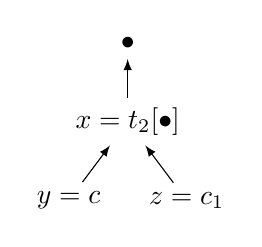
\begin{tikzpicture}[ 
  edge from parent path={(\tikzchildnode\tikzchildanchor) edge [-latex] (\tikzparentnode\tikzparentanchor)},
  level distance=1cm
]
\node (d) {$\bullet$} child{node (a) {$x=t_2[\bullet]$} child{node (b) {$y=c$}} child{node (c)
{$z=c_1$}}};

\end{tikzpicture}
\end{center}
In this scheme, each environment is represented by a linked list, with
the binding of $x$ shared between them. This simple example
illustrates a shared, linked environment ~\cite{appel1988optimizing}
and dates back to Landin's SECD machine~\cite{landin1964mechanical}.

The strengths and weaknesses of each approach are well known.  With a flat
environment variable lookup is implemented by a simple offset, or even
bound to a particular register~\cite{jonesstg, appel2006compiling},
but significant duplication can occur.  In a shared environment, unnecessary
duplication is avoided, but a cost is incurred on dereference whenever the
link structure must be traversed.

\subsection{Call-By-Need and the Heap}

Historically, flat environments have dominated call-by-need implementations
\cite{jonesstg, TIM, johnsson1984efficient,
boquist1997grin}. We speculate that this is in part because call-by-need
evaluation has historically been implemented with combinators, which take all
their free variables as formal parameters, and therefore suit flat environments
well. Note that for call-by-need languages, one must be careful when using flat
environments.  Because results from bound computations have to be shared across
closures referencing them, an implementation of call-by-need cannot copy
closures across environments. To illustrate this, consider again the earlier
example.  If we copied closures, results from evaluation of $t_2[\bullet]$ from
dereferencing $x$ in $t$ would not be shared with the instances of $x$ in
$t_1$.  This is fine for call-by-name, but to implement call by need, we must
ensure sharing.

The standard approach is to add a heap, which maps addresses to closures
\cite{jonesstg, TIM, johnsson1984efficient, sestoft} and then
modify the environments to map variables to addresses in the heap. The final
step adds update markers pointing to heap addresses on the stack, to update
the closures at those locations in the heap with their value once they have been
evaluated.  Reconsidering the shared environment diagram from the preceding
section, if we updated the $x=t_2[\bullet]$ with $t_2[\bullet]$'s corresponding
value after it was entered, the result would be shared between $t$ and $t_2$
without an additional heap. This is what we now describe and implement.

\section{Shared Environment Call-By-Need} \label{sec:calc}

Here we describe the key idea of our approach, showing how
the shared environment described earlier can be applied to call-by-need
evaluation. We start with a well-known abstract machine for evaluating
call-by-name, the Krivine machine $K$, Figure~\ref{fig:Krivine}.
The mechanics are simple: applications push their argument onto the stack,
abstractions pull an argument off the stack and move it into the environment,
and variables enter the closure at their index into the environment.

\begin{figure}
\textbf{Syntax}
\begin{align*}
\tag{State} s &::= \langle c, \sigma \rangle \\
\tag{Closure} c &::= t [\rho] \\
\tag{Environment} \rho &::= \bullet \; | \; c \cdot \rho \\
\tag{Context} \sigma &::= \square \; | \; \sigma \; c  \\
\end{align*}
\textbf{Semantics}
\begin{align*}
\tag{Lam}
\langle \lambda t[\rho], \sigma \; c \rangle 
  &\rightarrow_{K}
\langle t[c \cdot \rho], \sigma \rangle  \\
\tag{App}
\langle t \; t'[\rho], \sigma \rangle
  &\rightarrow_{K}
\langle t[\rho], \sigma \; t'[\rho] \rangle \\
\tag{Var1}
\langle 0[c \cdot \rho ], \sigma  \rangle
  &\rightarrow_{K}
\langle c, \sigma \rangle  \\
\tag{Var2}
\langle i[c \cdot \rho], \sigma \rangle
  &\rightarrow_{K}
\langle (i-1)[\rho], \sigma \rangle \\
\end{align*}
\caption{Syntax and semantics of the call-by-name $K$ machine.}
\label{fig:Krivine}
\end{figure}


Note that we have not specified how the environment is represented in the $K$
machine. To move towards the goal of sharing via environment structure,
we force the environment to be shared by creating a heap of environment
cells, and then extending each cell manually. This produces the $K'$ machine,
Figure~\ref{fig:K'}.

\begin{figure*}
\textbf{Syntax}
\begin{align*}
\langle c, \sigma, \mu f \rangle &\rightarrow_{K'} \langle c, \sigma, \mu, f \rangle \\
\tag{Closure} c &::= t [l] \\
\tag{Heap} \mu &::= \epsilon \; | \; \mu [ l \mapsto \rho ] \\
\tag{Environment} \rho &::= \bullet \; | \; c \cdot l \\
\tag{Context} \sigma &::= \square \; | \; \sigma \; c \\
\tag{Location} l,u,f &\in \mathbb{N}
\end{align*}
\textbf{Semantics}
\begin{align*}
\tag{Lam}
\langle \lambda t[l], \sigma \; c, \mu, f \rangle 
  &\rightarrow_{K'}
\langle t[f], \sigma, \mu[f \mapsto c \cdot l], f+1 \rangle  \\
\tag{App}
\langle t \; t'[l], \sigma, \mu, f \rangle
  &\rightarrow_{K'}
\langle t[l], \sigma \; t'[l], \mu, f \rangle \\
\tag{Var1}
\langle 0[l], \sigma, \mu, f \rangle
  &\rightarrow_{K'}
\langle c, \sigma, \mu, f \rangle 
\; \textnormal{where} \; c \cdot l' = \mu(l)\\
\tag{Var2}
\langle i[l], \sigma, \mu, f \rangle
  &\rightarrow_{K'}
\langle (i-1)[l'], \sigma, \mu, f \rangle
\; \textnormal{where} \; c \cdot l' = \mu(l) \\
\end{align*}
\caption{Syntax and semantics of the call-by-name $K'$ machine.}
\label{fig:K'}
\end{figure*}


Now, we have a heap of environments, which ensures that the
environments are shared when extended.  The $K'$ machine is identical to the $K$
machine, except that it forces this sharing of environments. 

Our explicitly shared environments enable us to add the necessary
machinery to implement full call-by-need semantics. We modify the $K'$ machine
to make it lazy in much the same way as Sestoft modified the Krivine
machine~\cite{sestoft}. We add update markers so that when a closure is entered,
the Var1 rule pushes an update marker to the corresponding location onto the
stack.  Then, when the corresponding value is our current closure, it will pop
the update marker, and replace the closure on the heap with itself. This
call-by-need $L$ machine is specified in Figure~\ref{fig:L}.

\begin{figure*}
\textbf{Syntax}
\begin{align*}
\tag{Closure} c &::= t [l] \\
\tag{Heap} \mu &::= \epsilon \; | \; \mu [ l \mapsto \rho ] \\
\tag{Environment} \rho &::= \bullet \; | \; c \cdot l \\
\tag{Value} v &::= \lambda t[l] \\
\tag{Context} \sigma &::= \square \; | \; \sigma \; c \;  | \; u:=\sigma \\
\tag{Location} l,u,f &\in \mathbb{N}
\end{align*}
\textbf{Semantics}
\begin{align*}
\tag{Upd}
\langle v, u := \sigma, \mu[u \mapsto c \cdot l], f \rangle 
  &\rightarrow_{\mathcal{CE}} 
\langle v, \sigma, \mu[u \mapsto v \cdot l], f \rangle  \\
\tag{Lam}
\langle \lambda t[l], \sigma \; c, \mu, f \rangle 
  &\rightarrow_{\mathcal{CE}}
\langle t[f], \sigma, \mu[f \mapsto c \cdot l], f+1 \rangle  \\
\tag{App}
\langle t \; t'[l], \sigma, \mu, f \rangle
  &\rightarrow_{\mathcal{CE}}
\langle t[l], \sigma \; t'[l], \mu, f \rangle \\
\tag{Var1}
\langle 0[l], \sigma, \mu, f \rangle
  &\rightarrow_{\mathcal{CE}}
\langle c, \sigma, \mu, f \rangle 
\; \textnormal{where} \; c \cdot l' = \mu(l)\\
\tag{Var2}
\langle i[l], \sigma, \mu, f \rangle
  &\rightarrow_{\mathcal{CE}}
\langle (i-1)[l'], \sigma, \mu, f \rangle
\; \textnormal{where} \; c \cdot l' = \mu(l) \\
\end{align*}
\caption{Syntax and semantics of the call-by-need $\mathcal{CE}$ machine.}
\label{fig:L}
\end{figure*}


We see from the semantics that all that has changed between the $K'$ and the
$L$ machine is the addition of the update marker to the Context
(which can be implemented as a normal stack), and the corresponding Update and
Var1 rules. This is in contrast to flat environment machines, such as the TIM~\cite{TIM}, which require more
complex machinery to ensure proper sharing.

Our $L$ machine is similar to existing lazy variants of the Krivine machine,
such as that defined by Sestoft \cite{sestoft}, except that instead of leaving
the environment structure unspecified, and adding a heap of closures, we have
forced the environment to be shared, and used that shared environment to
implement the necessary sharing of results.\footnote{In fact, in the code
comments of his dissertation, Sestoft mentions possible environment sharing, but
it is never formalized.} 

\section{An Example}

We now turn to visualizations of example executions to provide intuition for how
the $L$ machine operates. Figure~\ref{fig:states} shows a portion of the
execution trace during the evaluation of $(\lambda a.(\lambda b.b \; a) (\lambda
c.c \; a)) ((\lambda i.i) (\lambda j.j))$. 

\begin{figure*}
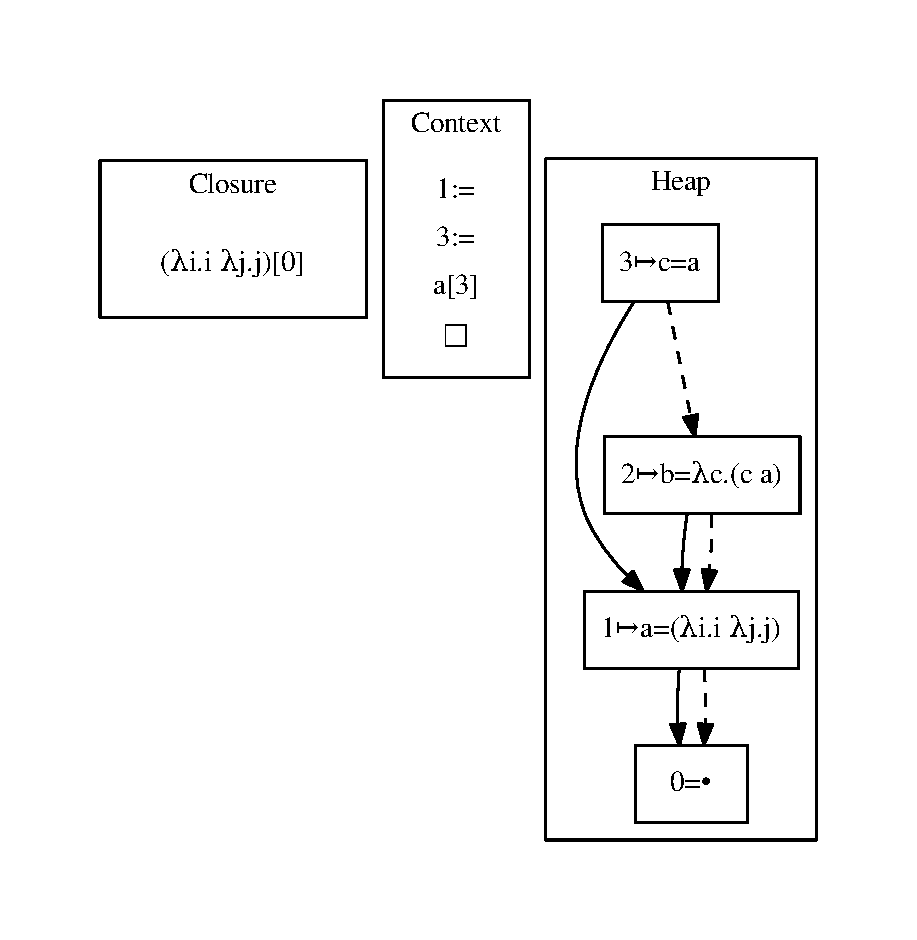
\includegraphics[width=\linewidth/3]{figures/12.pdf}
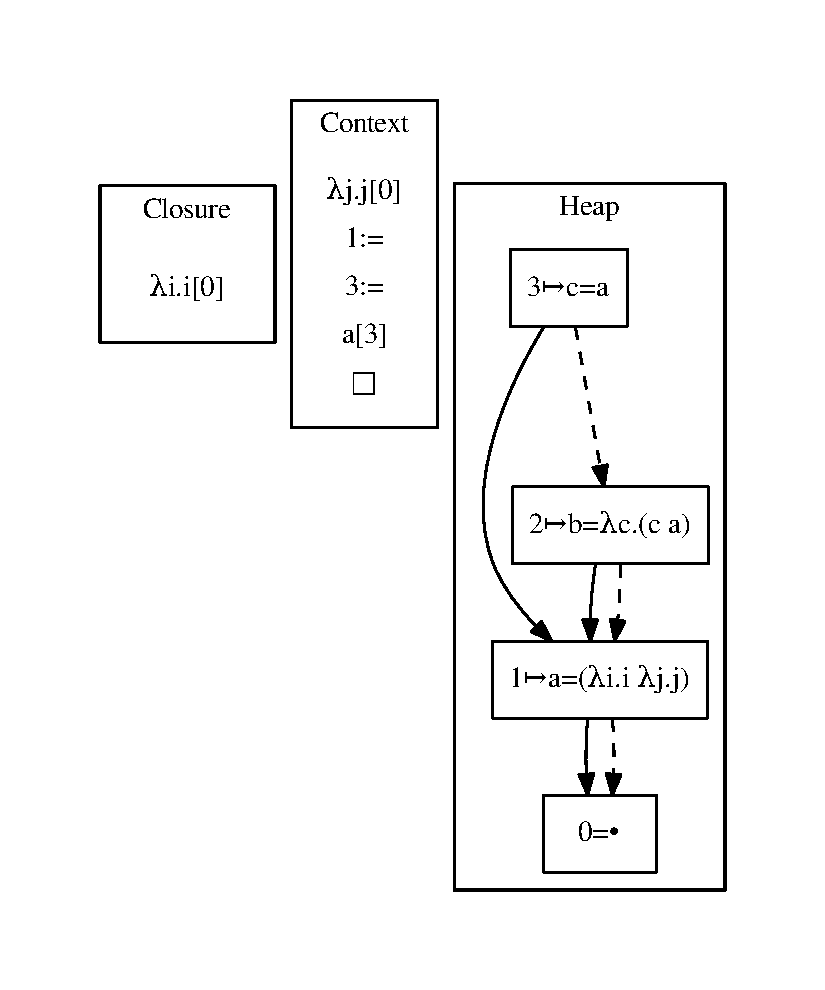
\includegraphics[width=\linewidth/3]{figures/13.pdf}
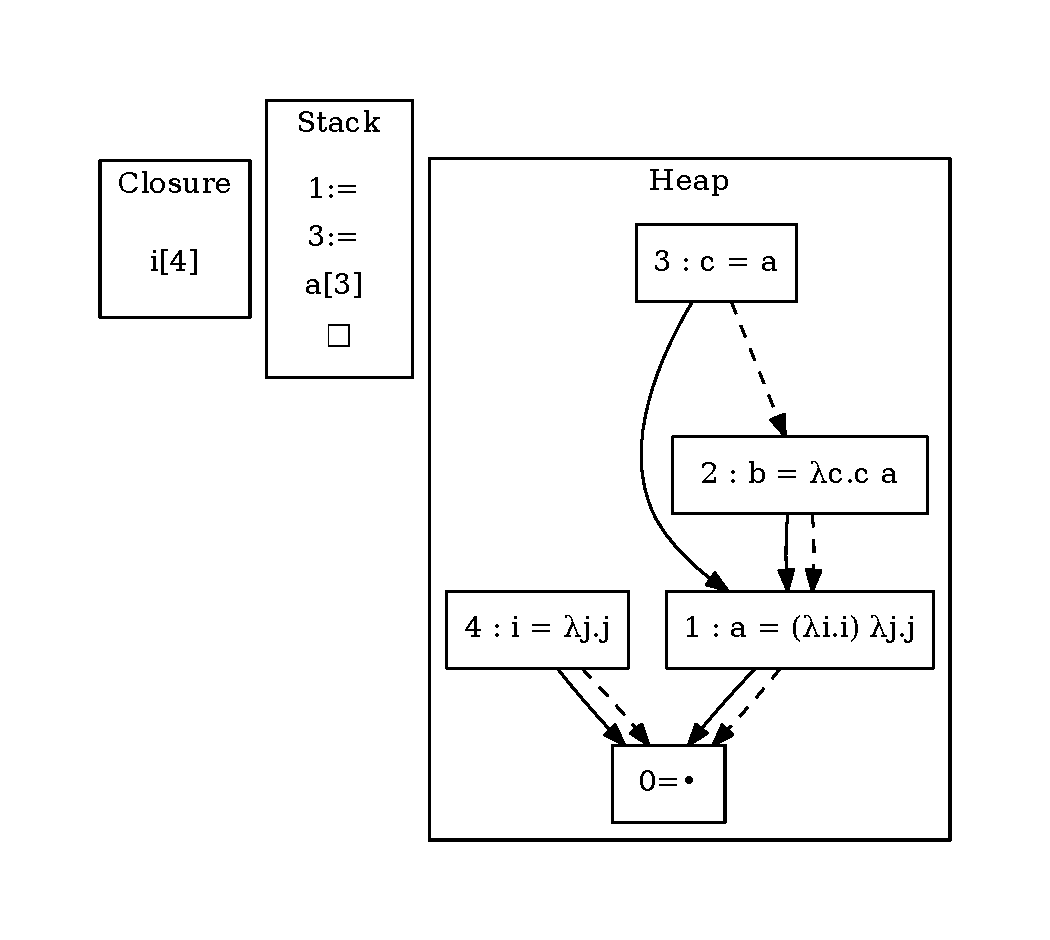
\includegraphics[width=\linewidth/3]{figures/14.pdf}
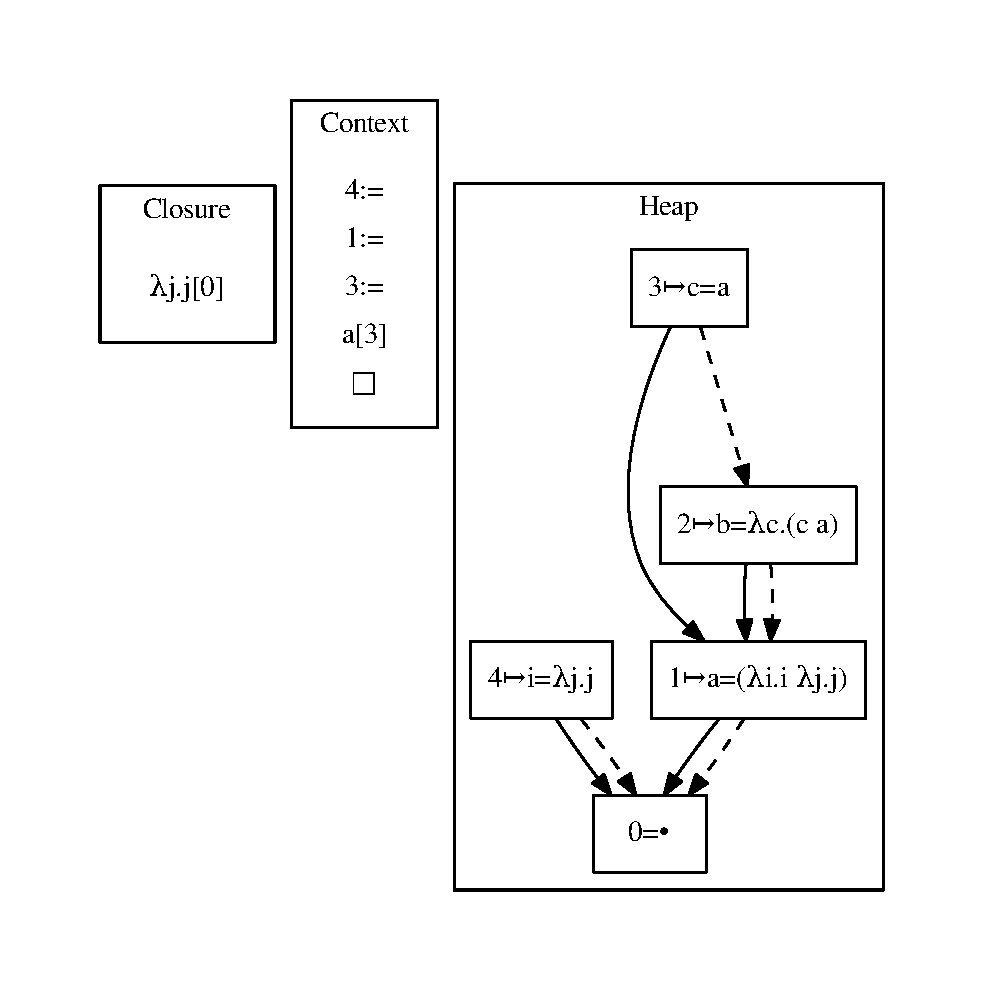
\includegraphics[width=\linewidth/3]{figures/15.pdf}
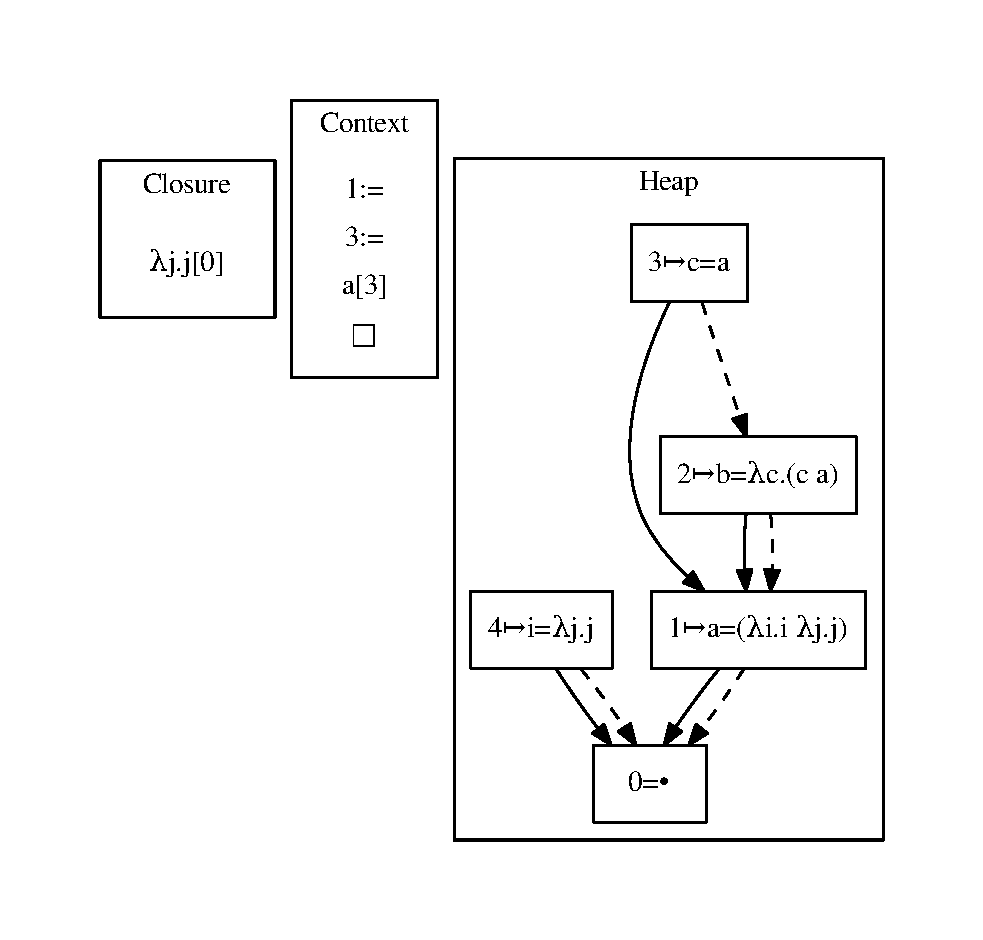
\includegraphics[width=\linewidth/3]{figures/16.pdf}
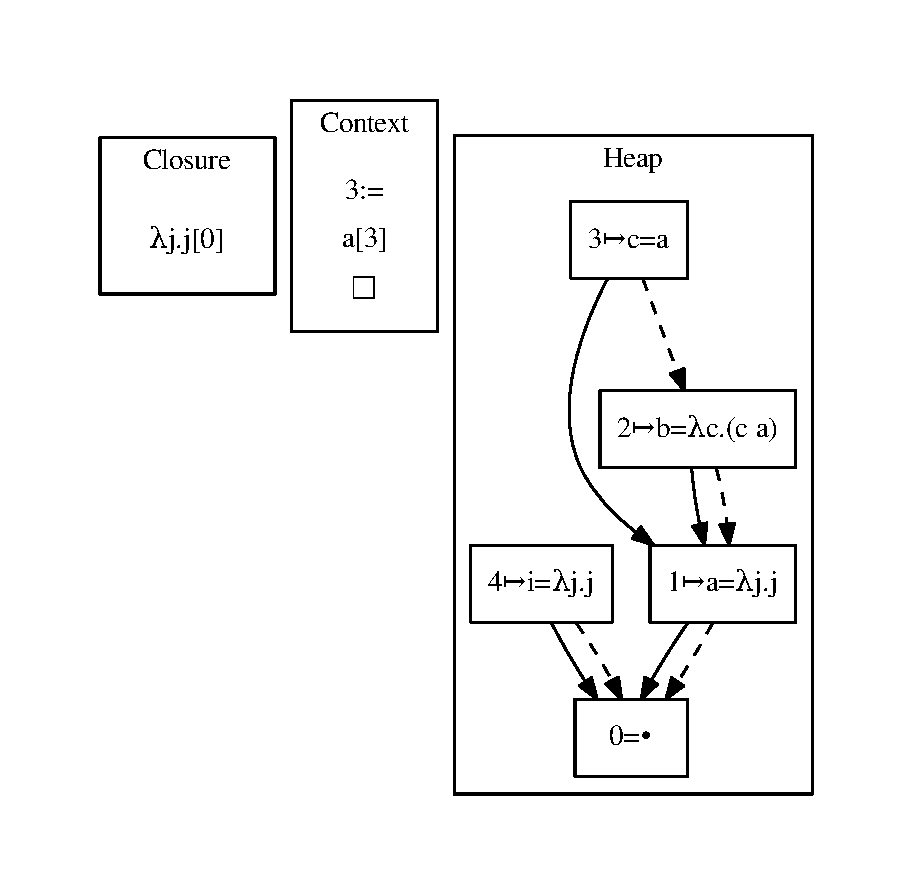
\includegraphics[width=\linewidth/3]{figures/17.pdf}
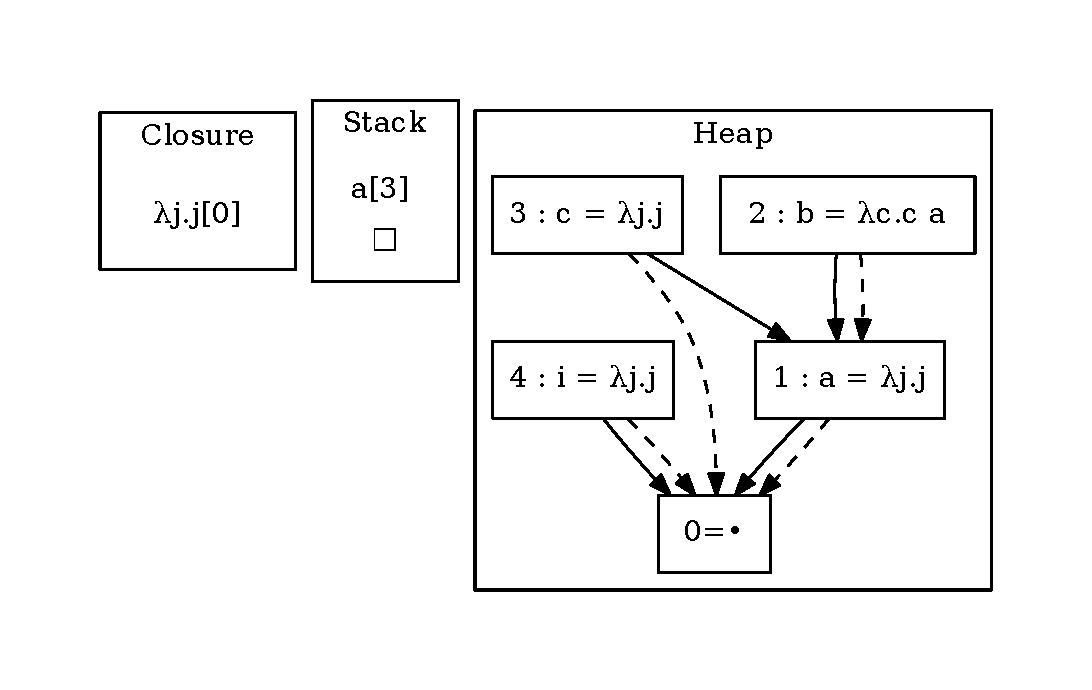
\includegraphics[width=\linewidth/3]{figures/18.pdf}
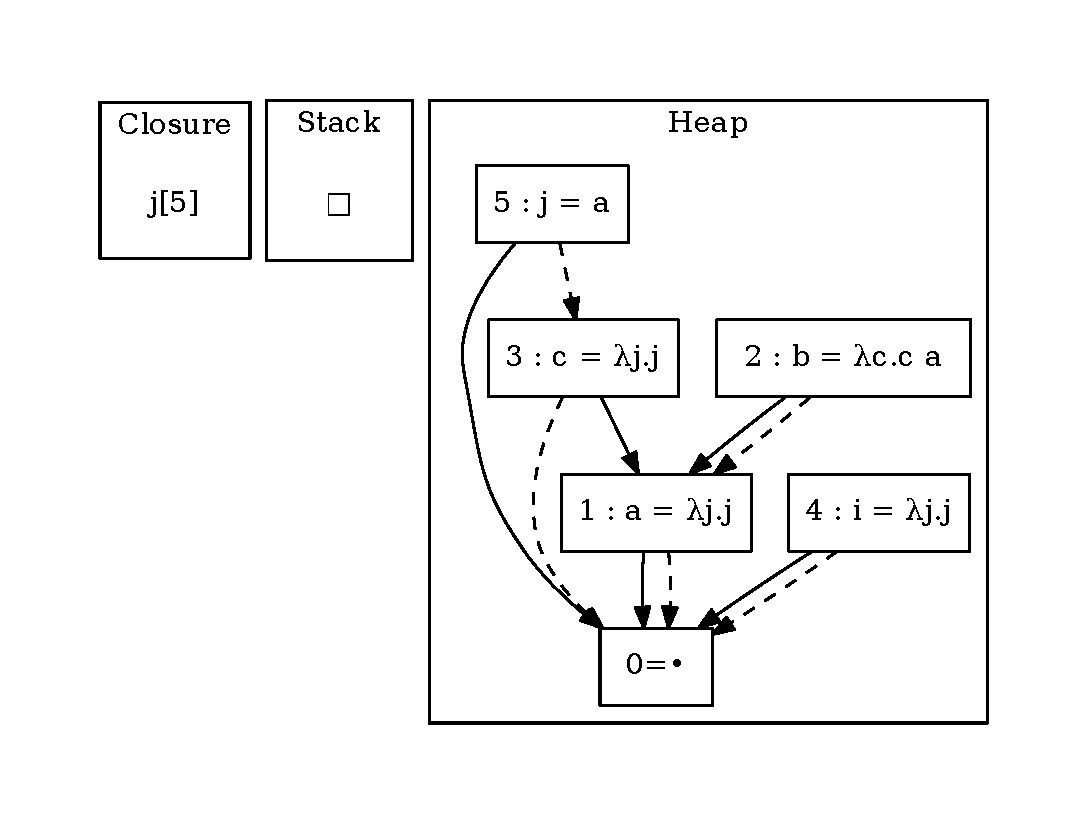
\includegraphics[width=\linewidth/3]{figures/19.pdf}
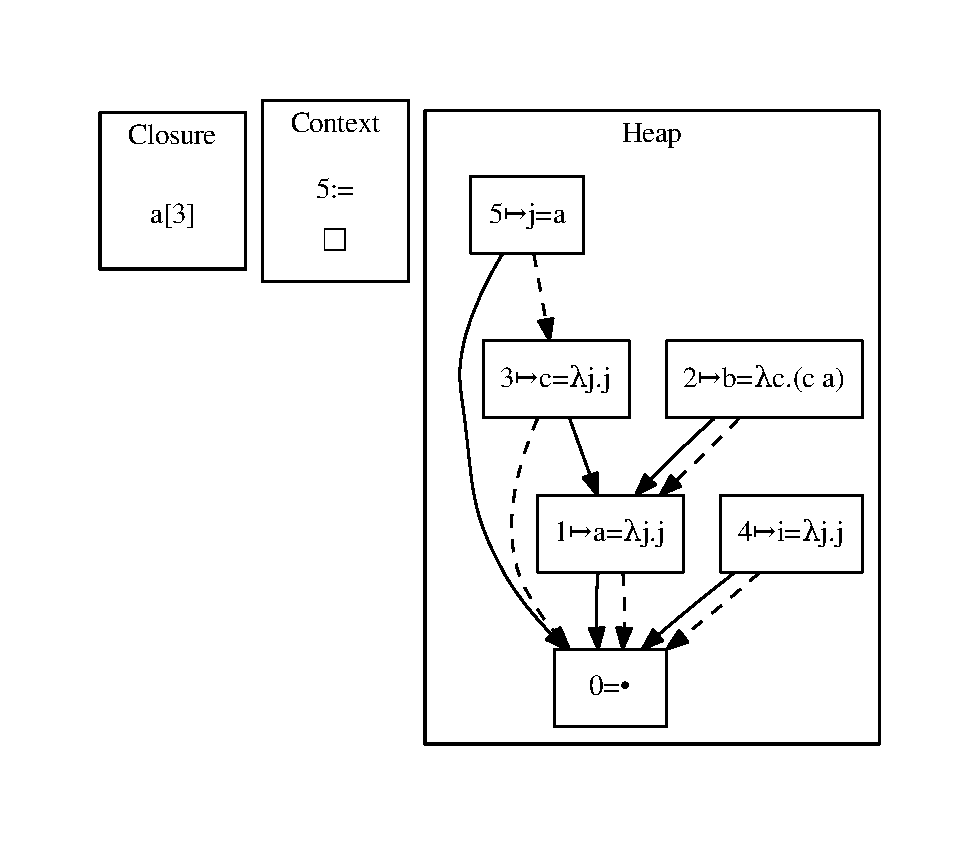
\includegraphics[width=\linewidth/3]{figures/20.pdf}
\caption{An example sequence of machine states during the evaluation of the term
$(\lambda a.(\lambda b.b \; a) (\lambda c.c
\; a)) ((\lambda i.i) (\lambda j.j))$. Order is left to right, top to bottom.
The free heap location $f$ is left out to save space. Dotted lines denote
the pointer for the closure's environment at a cell, and solid lines denote the
environment continuation. For example, in the first state, the environment
defined at location 3 corresponds to $c = a \cdot a = (\lambda i.i) \lambda j.j \cdot
\bullet$ in the $K$ machine's environment definition. We see the update rule in
effect when }
\label{fig:states}
\end{figure*}


We can see each rule in effect in our visualization, and how it changes the
state of the machine, directly. Hopefully this gives the reader some intiution
for how the machine operates, and how simple its rules are from a mechanical
point of view. 

[THIS IS NOT ENOUGH. You can't expect the reader to follow the diagrams
without any guidance. Include a narrative explanation of the whole figure here. You have enough
space for the figure caption on this page.]

\section{Correspondence to Call-By-Need Lambda Calculus}
To convince ourselves that the call-by-need
semantics are correctly implemented, we turn to the work of
Ariola et al.\cite{ariola1995call}, which specified an operational semantics for
call-by-need lambda calculus, Figure~\ref{fig:cbn}.

\begin{figure}
\begin{align*}
\tag{Id} \inference
{\langle \Phi \rangle e \Downarrow \langle \Psi \rangle \lambda x.e'}
{\langle \Phi, x \mapsto e, \Upsilon \rangle x \Downarrow \langle \Psi, x
\mapsto \lambda x.e', \Upsilon \rangle \lambda x.e'}
\end{align*}
\begin{align*}
\tag{Abs} \inference 
{}
{\langle \Phi \rangle \lambda x . e \Downarrow \langle \Phi \rangle \lambda x.e}
\end{align*}
\begin{align*}
\tag{App} \inference
{\langle \Phi \rangle e_l \Downarrow \langle \Psi \rangle \lambda 
x.e_n \\ \langle \Psi, x' \mapsto e_m \rangle [x'/x]e_n \Downarrow \langle
\Upsilon \rangle \lambda y.e'}
{\langle \Phi \rangle e_l \; e_m \Downarrow \langle \Upsilon \rangle \lambda y.e'}
\end{align*}
\caption{Ariola et al.'s Call-By-Need Operational Semantics (Figure 8 of Ref.~\cite{ariola1995call})}
\label{fig:cbn}
\end{figure}


Case-wise induction on $\rightarrow_{N}$ gives an ordering to the closures in
the cactus environment. This is similar to the ordering from Lemma 8.1 of
Ref.~\cite{ariola1995call}.  Using this ordering, we define the function
$flatten$, which takes any $(c, \mu)$ and flattens it accordingly. It does so by
mapping any $(c, \mu)$ to a $\langle \Phi \rangle t$, with the necessary
variable hygiene. With this function, along with structural induction on term
size, it is not hard to show that $\rightarrow_{L}$ bisimulates $\downarrow$.

Ariola et al.'s semantics throws out environment structure because it doesn't
need to keep it. Similarly the abstract machines derived from the semantics
(e.g., \cite{garcia2009lazy}) are forced to search for variables in the
environment---deBruijn indices are not an option. In contrast, our
machine retains that structure in the cactus environment, which allows the use
of deBruijn indices and a straighforward low-level implementation (next
section).

\section{Implementation}\label{sec:impl}

First, some preliminaries. We target the x64 GNU assembler running on
Linux. Any x64 linux machine that has GNU ld should be able to run the
compiled examples.  We include in the data type a label for each basic
block so it can be jumped to directly, and we annotate each x64
instruction line with a comment summarizing its purpose.  We also
explain the simple mapping between each basic block and the
corresponding rule from the abstract machine specification.

The compile function takes a deBruijn indexed lambda term and
generates a list of basic blocks of x64 assembly code. In the case of the Var1
and Var2 rules, they are combined into a single basic block, which traverses the
environment linked list until it reaches a closure, then pushes an update marker
to that location. The App rule is the simplest: it consists of two instructions
that push the location of the argument term along with the current environment
pointer onto the stack. The Lam and Update rules are a little more complicated.
Recall that there is no rule in which we have a lambda as our current term, and
an empty stack. That is so, because that is the condition for termination. Thus, we
must add a check to see if the stack is empty (\texttt{checkTermBB}), and terminate if it
is (\texttt{termBB}). If it is not, then we check (\texttt{checkUpdateBB})
to see if it is an update marker (which
we have designated to be the \texttt{NULL} pointer or 0, as there cannot be a valid code
pointer to that location), and if it is,
update the marker and continue without changing the current closure. If it is
not an update marker, it is an argument closure, so we pop to extend our current
environment with it. 

\begin{figure*}
\begin{code}
compile e = compile' 0 e where 
  compile' l e = case e of
    Var i -> [varBB l i]
    Lam b -> checkTermBB l 
           : termBB l 
           : checkUpdateBB l 
           : updateBB l 
           : takeBB l 
           : compile' (succ l) b
    App m n -> appBB l nlab : ms ++ ns where
      ms = compile' (succ l) m
      ns@((nlab,_):_) = compile' (succ l + length ms) n

type Location = Int

appBB :: Location -> Label -> BasicBlock
appBB l n = ("App_"++show l, 
  ["push %rax"                                      -- Push environment
  ,"push $"++n])                                    -- Push argument code

varBB :: Location -> Var -> BasicBlock
varBB l i = ("Var_"++show l,
  replicate i "movq 16(%rax), %rax"                 -- Index into environment
  ++ ["push %rax"                                   -- Push update location
     ,"push $0"                                     -- Push update marker
     ,"movq %rax, %rcx"                             -- \
     ,"movq 8(%rax), %rax"                          -- Load new Environment
     ,"jmp *(%rcx)"])                               -- Jump to new code

checkTermBB :: Location -> BasicBlock
checkTermBB l = ("CheckTerm_"++show l,
  ["cmp %rsp, %rbp"                                 -- Check if stack is empty
  ,"jne CheckUpdate_"++show l])                     -- If not empty, check updates

termBB :: Location -> BasicBlock
termBB l = ("Term_"++show l,
  ["movq $"++show l++", %rdi"                       -- \
  ,"movq $60, %rax"                                 -- Exit with label exitcode
  ,"syscall"])                                      -- / 

checkUpdateBB :: Location -> BasicBlock
checkUpdateBB l = ("CheckUpdate_"++show l,
  ["cmpq $0, (%rsp)"                                -- Check for update marker
  ,"jne Take_"++show l])                            -- If not update, proceed to take

updateBB :: Location -> BasicBlock
updateBB l = ("Update_"++show l,
  ["movq 8(%rsp), %rcx"                             -- \
  ,"movq $CheckTerm_"++show l++", "++"(%rcx)"       --  Replace code pointer
  ,"movq %rax, 8(%rcx)"                             --  Replace env pointer
  ,"add $16, %rsp"                                  --  Pop update 
  ,"jmp CheckTerm_"++show l])                       --  Continue with new stack
 
takeBB :: Location -> BasicBlock
takeBB l = ("Take_"++show l,
  ["pop (%rbx)"                                     -- Pop code into free heap cell
  ,"pop 8(%rbx)"                                    -- Pop env into free heap cell
  ,"movq %rax, 16(%rbx)"                            -- Point env to free heap cell
  ,"movq %rbx, %rax"                                -- /
  ,"add $24, %rbx"])                                -- Increment free heap cell

\end{code}
\caption{Full compiler implementation}
\label{fig:impl}
\end{figure*}


\section{Discussion}
The abstract machine as presented has some surprisingly nice properties and some
weaknesses. There is a sense in which the $L$ machine is \emph{lazier} than flat
environment implementations. Instead of spending time allocating a flat
environment to optimize variable lookup, our implementation does the minimal
amount of preparation work. Of course, this comes with the previously mentioned
cost of non-constant variable lookup time. 

We hope that this simple implementation could be of pedagogical value.
Furthermore, we believe it could make for a good target for abstraction thanks
to its simplicity, following the approach of Van Horn et
al\cite{van2010abstracting}. For example, its straightforward heap structure
could be amenable to abstraction, allowing for easier analysis of static heap
properties.

\section{Conclusion and Future Work}
We hope that the reader is convinced of the elegance of this approach to implementing
call-by-need, and that this use of shared environments can lead to
improved future implementations. We are not aware of any call-by-need
implementations that are as simple as the one described here.
Beyond simplicity and elegance, however, we are actively exploring compile-time
optimizations to make this abstract machine practically usable for lazy language
implementation. [ANYTHING ELSE?]

% We recommend abbrvnat bibliography style.
\bibliographystyle{abbrvnat}
\bibliography{annotated}

\end{document}

